\documentclass[border=5pt]{standalone}

\usepackage{amsfonts,amssymb,amsmath}
\usepackage{tikz}
\usetikzlibrary{matrix}

\newcommand{\RP}{\mathbb{RP}}
\newcommand{\CP}{\mathbb{CP}}

\tikzset{ 
table/.style={
  matrix of nodes,
  row sep=-\pgflinewidth,
  column sep=-\pgflinewidth,
  nodes={rectangle,text width=3em,align=center},
  text depth=1.25ex,
  text height=3.5ex,
  nodes in empty cells
},
row 1/.style={nodes={fill=gray!20,text depth=0.4ex,text height=3ex}},
row 11/.style={nodes={text depth=6ex,text height=4ex,execute at begin node=\setlength{\baselineskip}{4ex}}},
row 13/.style={nodes={text depth=6ex,text height=4ex,execute at begin node=\setlength{\baselineskip}{4ex}}},
row 14/.style={nodes={text depth=6ex,text height=4ex,execute at begin node=\setlength{\baselineskip}{4ex}}},
row 15/.style={nodes={text depth=13ex,text height=4ex,execute at begin node=\setlength{\baselineskip}{4ex}}},
column 1/.style={nodes={rectangle, text width=1cm, align=center}},
column 2/.style={nodes={rectangle, text width=14cm, align=left}},
column 3/.style={nodes={rectangle, text width=1cm, align=center}},
column 3/.style={nodes={rectangle, text width=2cm, align=center}},
row 16/.style={nodes={fill=gray!10,text depth=0.4ex,text height=3ex, align=center}}
}

\begin{document}
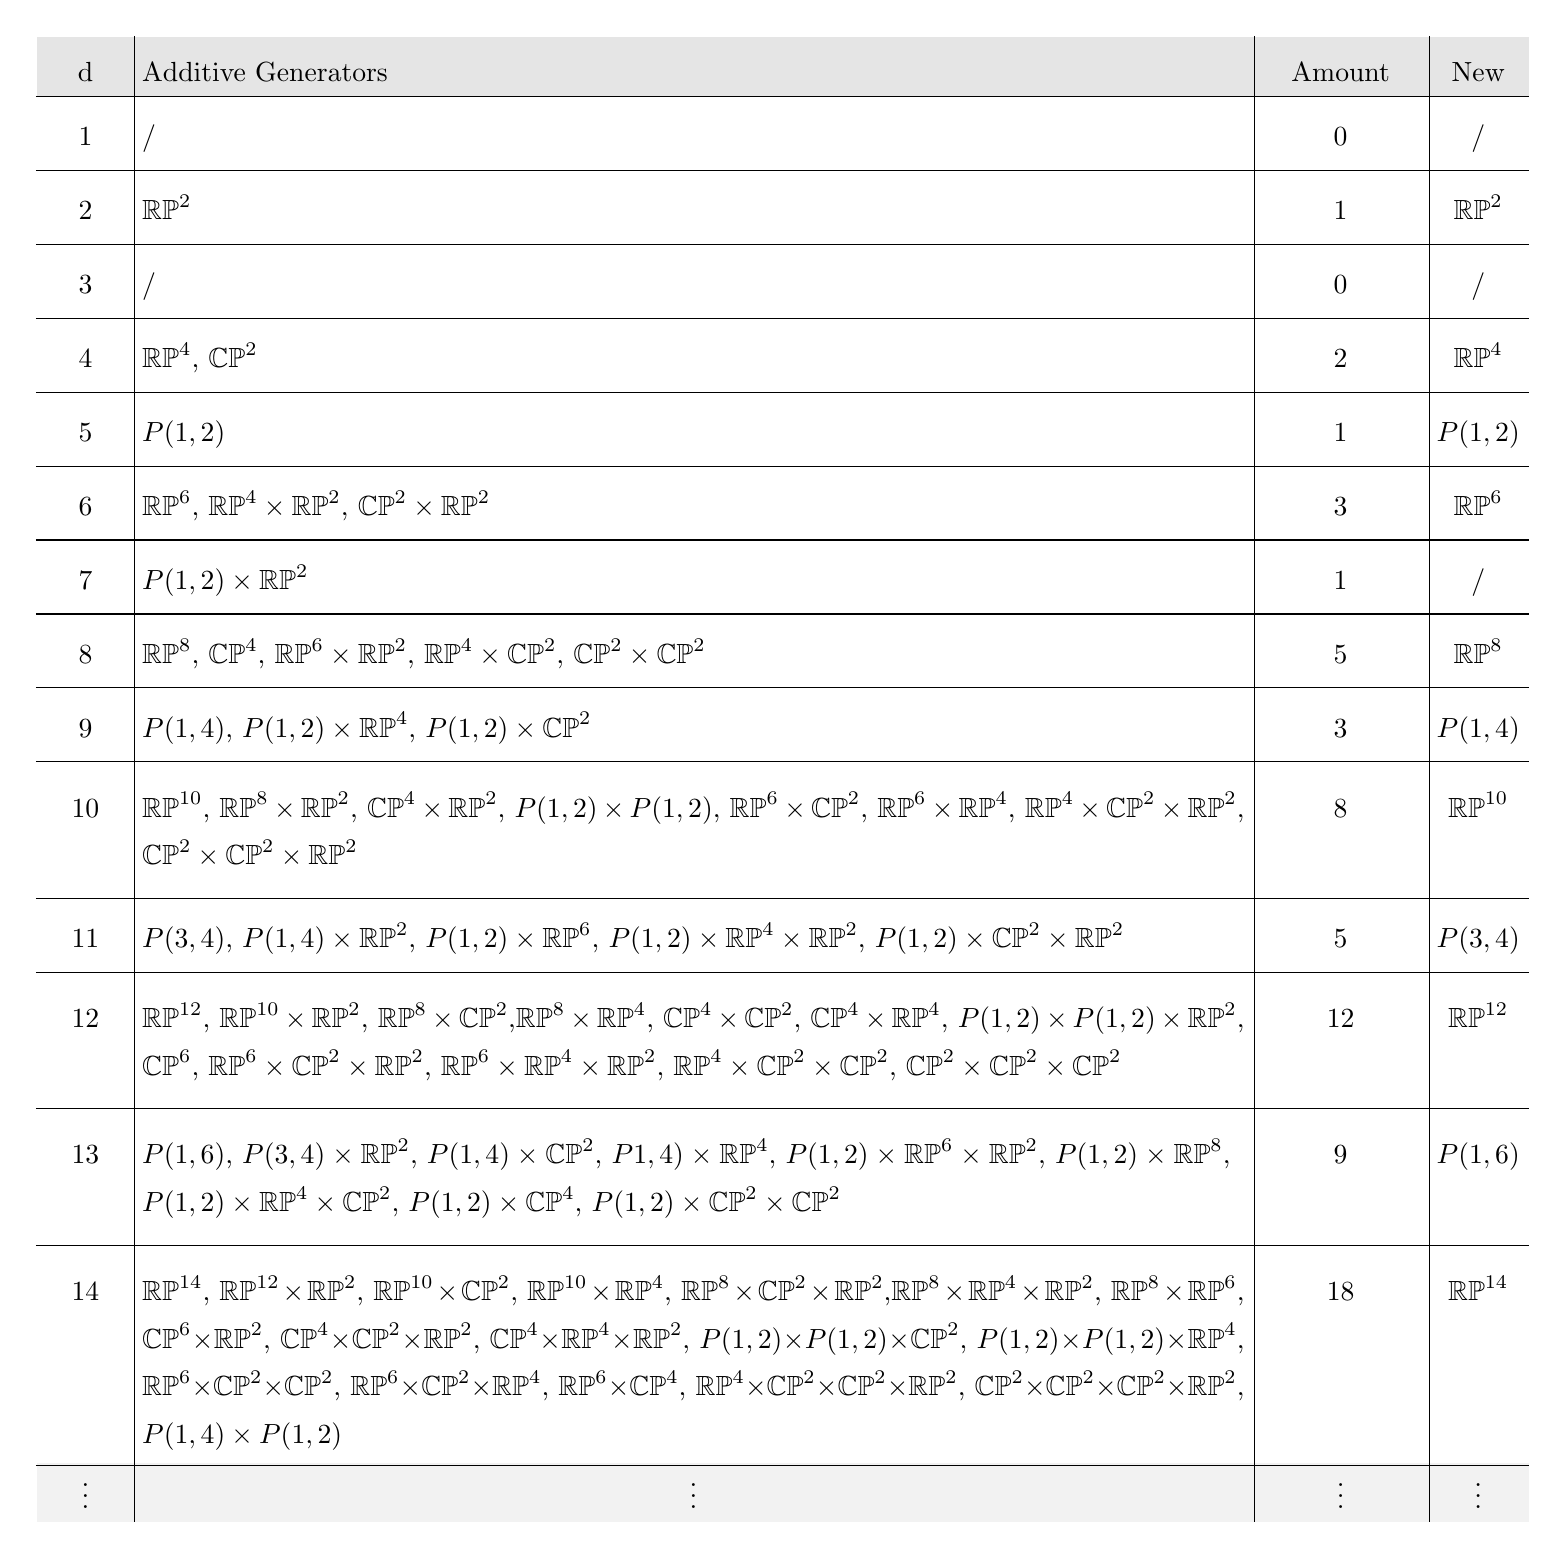
\begin{tikzpicture}
\matrix (mat) [table] {
    d & Additive Generators & Amount & New \\
    1 & $/$ & 0 & $/$ \\
    2 & $\RP^2$ & 1 & $\RP^2$ \\
    3 & $/$ & 0 & $/$ \\
    4 & $\RP^4$, $\CP^2$ & 2 & $\RP^4$ \\
    5 & $P(1,2)$ & 1 & $P(1,2)$ \\
    6 & $\RP^6$, $\RP^4\times\RP^2$, $\CP^2\times\RP^2$ & 3 & $\RP^6$ \\
    7 & $P(1,2)\times\RP^2$ & 1 & $/$ \\
    8 & $\RP^8$, $\CP^4$, $\RP^6\times\RP^2$, $\RP^4\times\CP^2$, $\CP^2\times\CP^2$ & 5 & $\RP^8$ \\
    9 & $P(1,4)$, $P(1,2)\times\RP^4$, $P(1,2)\times\CP^2$ & 3 & $P(1,4)$ \\
    10 & $\RP^{10}$, $\RP^8\times\RP^2$, $\CP^4\times\RP^2$, $P(1,2)\times P(1,2)$, $\RP^6\times\CP^2$, $\RP^6\times\RP^4$, $\RP^4\times\CP^2\times\RP^2$, $\CP^2\times\CP^2\times\RP^2$ & 8 & $\RP^{10}$ \\
    11 & $P(3,4)$, $P(1,4)\times\RP^2$, $P(1,2)\times\RP^6$, $P(1,2)\times\RP^4\times\RP^2$, $P(1,2)\times\CP^2\times\RP^2$ & 5 & $P(3,4)$ \\
    12 & $\RP^{12}$, $\RP^{10}\times\RP^2$, $\RP^8\times\CP^2$,$\RP^8\times\RP^4$, $\CP^4\times\CP^2$, $\CP^4\times\RP^4$, $P(1,2)\times P(1,2)\times\RP^2$, $\CP^6$, $\RP^6\times\CP^2\times\RP^2$, $\RP^6\times\RP^4\times\RP^2$, $\RP^4\times\CP^2\times\CP^2$, $\CP^2\times\CP^2\times\CP^2$ & 12 & $\RP^{12}$ \\
    13 & $P(1,6)$, $P(3,4)\times\RP^2$, $P(1,4)\times\CP^2$, $P1,4)\times\RP^4$, $P(1,2)\times\RP^6\times\RP^2$, $P(1,2)\times\RP^8$, $P(1,2)\times\RP^4\times\CP^2$, $P(1,2)\times\CP^4$, $P(1,2)\times\CP^2\times\CP^2$ & 9 & $P(1,6)$ \\
    14 & $\RP^{14}$, $\RP^{12}\times\RP^2$, $\RP^{10}\times\CP^2$, $\RP^{10}\times\RP^4$, $\RP^8\times\CP^2\times\RP^2$,$\RP^8\times\RP^4\times\RP^2$, $\RP^8\times\RP^6$, $\CP^6\times\RP^2$, $\CP^4\times\CP^2\times\RP^2$, $\CP^4\times\RP^4\times\RP^2$, $P(1,2)\times P(1,2)\times\CP^2$, $P(1,2)\times P(1,2)\times\RP^4$, $\RP^6\times\CP^2\times\CP^2$, $\RP^6\times\CP^2\times\RP^4$, $\RP^6\times\CP^4$, $\RP^4\times\CP^2\times\CP^2\times\RP^2$, $\CP^2\times\CP^2\times\CP^2\times\RP^2$, $P(1,4)\times P(1,2)$ & 18 & $\RP^{14}$ \\
    $\vdots$ & $\vdots$ & $\vdots$ & $\vdots$\\
};
% the matrix rules
\foreach \x in {1,...,15}
{
  \draw
    ([xshift=-.5\pgflinewidth]mat-\x-1.south west) --
    ([xshift=-.5\pgflinewidth]mat-\x-4.south east);
  }
\draw
    ([yshift=.5\pgflinewidth]mat-1-3.north east) --
    ([yshift=.5\pgflinewidth]mat-16-3.south east);
\draw
    ([yshift=.5\pgflinewidth]mat-1-2.north east) --
    ([yshift=.5\pgflinewidth]mat-16-2.south east);
\draw
    ([yshift=.5\pgflinewidth]mat-1-1.north east) --
    ([yshift=.5\pgflinewidth]mat-16-1.south east);
\end{tikzpicture}
\end{document}
